\chapter{Populatiegenetica en natuurlijke selectie}\label{ch:b2:population-genetics}

In 1848 werd bij Manchester een zwarte berkenspanner gevangen; in 1895 waren
negentien van de twintig nachtvlinders in de stad zwart, en in 1970, toen het
roet verdween, was de lichte vorm terug. De vlinders veranderden niet: de
verhoudingen van twee \omterm{def:b2:meiosis-heredity:vocabulary}{allelen} in een populatie van miljoenen veranderden,
onder de ogen van vogels, in enkele tientallen generaties. Darwin had gezien
dat selectie soorten moet veranderen, maar had geen manier om haar te tellen;
dat tellen is de \omterm{def:b2:population-genetics:frequencies}{populatiegenetica}, en het is het rekenwerk van dit hoofdstuk.
Ze vraagt hoe \omterm{def:b2:population-genetics:frequencies}{allelfrequenties} zich gedragen wanneer er niets op inwerkt, en
daarna hoe snel selectie, \omterm{def:b2:genome-diversification:mutation}{mutatie}, migratie, toeval en inteelt ze verschuiven
--- en ze eindigt met de kenmerken die niet door één gen maar door vele worden
bepaald, en dat is het meeste van wat selectie werkelijk ziet.

\section{De genenpool in rust}

\begin{definition}[Populatie, genenpool, frequenties]\label{def:b2:population-genetics:frequencies}
\index{populatiegenetica}\index{genenpool}\index{allelfrequentie}
Een \emph{populatie} is een groep individuen van één soort die onderling
voortplanten; haar \emph{genenpool} is de verzameling van al hun \omterm{def:b2:meiosis-heredity:vocabulary}{allelen}.
Voor een locus met twee \omterm{def:b2:meiosis-heredity:vocabulary}{allelen} $A$ en $a$ in een diploïde populatie van
$N$ individuen zijn de \emph{allelfrequenties} $p = (2N_{AA} +
N_{Aa})/2N$ en $q = 1 - p$, en de \emph{genotypefrequenties} zijn
de fracties $AA$, $Aa$ en $aa$. Evolutie, in de engste zin, is een
verandering van allelfrequenties tussen generaties; de vraag van dit hoofdstuk
is wat ze verandert en hoeveel.
\end{definition}

\begin{theorem}[Hardy--Weinberg]\label{thm:b2:population-genetics:hw}
\index{wet van Hardy--Weinberg}
In een grote populatie met willekeurige paring, zonder selectie, \omterm{def:b2:genome-diversification:mutation}{mutatie}
of migratie, veranderen de \omterm{def:b2:population-genetics:frequencies}{allelfrequenties} niet van de ene generatie op de
volgende, en na één enkele generatie van willekeurige paring zijn de
genotypefrequenties
\[
AA : p^{2}, \qquad Aa : 2pq, \qquad aa : q^{2},
\]
en blijven ze zo. Dominantie laat een \omterm{def:b2:meiosis-heredity:vocabulary}{dominant} \omterm{def:b2:meiosis-heredity:vocabulary}{allel} zich niet verspreiden,
en een zeldzaam \omterm{def:b2:meiosis-heredity:vocabulary}{recessief} \omterm{def:b2:meiosis-heredity:vocabulary}{allel} gaat niet verloren: het verbergt zich in
heterozygoten, die de homozygoten met $2p/q$ tegen één overtreffen --- voor
$q = 0.01$ tweehonderd tegen één. De wet is de nulhypothese van de
\omterm{def:b2:population-genetics:frequencies}{populatiegenetica}: een afwijking ervan in een echte populatie, of een
verandering van $p$ tussen generaties, is het kenmerk van een van de
krachten hieronder.
\end{theorem}
\begin{proof}
Willekeurige paring is willekeurige versmelting van gameten: een gameet draagt
$A$ met kans $p$ en $a$ met kans $q$, onafhankelijk van zijn
partner, zodat de zygote $AA$ is met kans $p^{2}$, $Aa$ met
$2pq$, $aa$ met $q^{2}$. De \omterm{def:b2:population-genetics:frequencies}{allelfrequentie} in de volgende
generatie is $p' = p^{2} + \tfrac12(2pq) = p(p + q) = p$: onveranderd.
Omdat de genotypefrequenties alleen van $p$ afhangen, zijn ze in elke
generatie na de eerste dezelfde.
\end{proof}

\begin{example}[Een frequentie aflezen]\label{ex:b2:population-genetics:cf}
Taaislijmziekte, \omterm{def:b2:meiosis-heredity:vocabulary}{recessief}, treft één Europees kind op 2500:
$q^{2} = 1/2500$, $q = 0.02$, en de dragersfrequentie is $2pq
\approx 0.04$ --- één persoon op 25 draagt een \omterm{def:b2:meiosis-heredity:vocabulary}{allel} dat zijn
homozygoten doodt, en \qty{98}{\%} van de kopieën van het \omterm{def:b2:meiosis-heredity:vocabulary}{allel} zit in
gezonde dragers, waar selectie ze niet kan zien. Daarom wordt een letaal
\omterm{def:b2:meiosis-heredity:vocabulary}{recessief} \omterm{def:b2:meiosis-heredity:vocabulary}{allel} zo traag verwijderd, en daarom hadden eugenetische plannen om
recessieve ziekten uit te roeien door de getroffenen te steriliseren nooit
kunnen werken: het rekenwerk van de volgende paragraaf laat zien hoe traag.
\end{example}

\section{Selectie}

\begin{definition}[Fitness]\label{def:b2:population-genetics:fitness}
\index{fitness}\index{selectiecoëfficiënt}
De \emph{fitness} $w$ van een \omterm{def:b2:meiosis-heredity:vocabulary}{genotype} is zijn relatieve bijdrage aan
nakomelingen voor de volgende generatie --- overleving tot de voortplanting
maal vruchtbaarheid, geschaald zodat het beste \omterm{def:b2:meiosis-heredity:vocabulary}{genotype} $w = 1$ heeft. De
\emph{selectiecoëfficiënt} $s$ van een \omterm{def:b2:meiosis-heredity:vocabulary}{genotype} is zijn tekort,
$w = 1 - s$. Fitness is een eigenschap van een \omterm{def:b2:meiosis-heredity:vocabulary}{genotype} in een omgeving,
niet van een \omterm{def:b2:meiosis-heredity:vocabulary}{allel} op zich: het \omterm{def:b2:meiosis-heredity:vocabulary}{allel} van de melanistische vlinder had $w > 1$
ten opzichte van het lichte op beroete schors en $w < 1$ op korstmos.
\end{definition}

\begin{theorem}[Selectie verandert de allelfrequentie]\label{thm:b2:population-genetics:selection}
\index{natuurlijke selectie!vergelijking}
Met genotypefitnesses $w_{AA}$, $w_{Aa}$, $w_{aa}$ is de gemiddelde
\omterm{def:b2:population-genetics:fitness}{fitness} $\bar w = p^{2}w_{AA} + 2pq\,w_{Aa} + q^{2}w_{aa}$ en is de
\omterm{def:b2:population-genetics:frequencies}{allelfrequentie} in de volgende generatie
\[
p' = \frac{p^{2}w_{AA} + pq\,w_{Aa}}{\bar w}, \qquad
\Delta p = p' - p = \frac{pq\,\bigl[p(w_{AA} - w_{Aa}) + q(w_{Aa} - w_{aa})\bigr]}{\bar w}.
\]
Twee gevolgen. Ten eerste is $\Delta p$ evenredig met $pq$: selectie
werkt het snelst bij tussenliggende frequenties en het traagst wanneer een
\omterm{def:b2:meiosis-heredity:vocabulary}{allel} zeldzaam of bijna gefixeerd is --- er is dan weinig variatie om op in te
werken. Ten tweede is de verandering tegen een \omterm{def:b2:meiosis-heredity:vocabulary}{recessief} \omterm{def:b2:meiosis-heredity:vocabulary}{allel} ($w_{AA} = w_{Aa} = 1$, $w_{aa} =
1 - s$) gelijk aan $\Delta q = -s\,pq^{2}/\bar w$, evenredig
met $q^{2}$: een zeldzaam \omterm{def:b2:meiosis-heredity:vocabulary}{recessief} \omterm{def:b2:meiosis-heredity:vocabulary}{allel} is voor selectie bijna onzichtbaar,
en het halveren van zijn frequentie vanaf $0.01$ duurt ongeveer honderd
generaties, zelfs wanneer zijn homozygoten letaal zijn. Een gunstig \omterm{def:b2:meiosis-heredity:vocabulary}{dominant}
\omterm{def:b2:meiosis-heredity:vocabulary}{allel} verspreidt zich eerst snel en stokt op het eind, om dezelfde
reden.
\end{theorem}
\begin{proof}
Van de nakomelingen is een fractie $p^{2}w_{AA}/\bar w$ van type $AA$ en
$2pq\,w_{Aa}/\bar w$ van type $Aa$ (de frequentie van elk \omterm{def:b2:meiosis-heredity:vocabulary}{genotype} gewogen naar
zijn \omterm{def:b2:population-genetics:fitness}{fitness} en opnieuw genormeerd); de $A$-allelen onder hen zijn alle van
de eerste en de helft van de tweede, wat $p'$ geeft. Aftrekken van $p =
p\bar w/\bar w$ en uitwerken van $\bar w$ geeft $\Delta p$. Voor een letaal
\omterm{def:b2:meiosis-heredity:vocabulary}{recessief} \omterm{def:b2:meiosis-heredity:vocabulary}{allel} ($s = 1$): $q' = q^{2}\cdot 0 + pq$ gedeeld door $\bar w = 1 -
q^{2}$, dus $q' = q/(1 + q)$, vandaar $1/q' = 1/q + 1$, en na $t$
generaties $1/q_t = 1/q_0 + t$: van $q_0 = 0.01$ tot $0.005$ duurt het
$t = 100$.
\end{proof}

\begin{omfigure}
\begin{tikzpicture}
\begin{axis}[
  width=0.8\linewidth, height=6cm,
  axis x line=bottom, axis y line=left,
  xmin=0, xmax=150, ymin=0, ymax=1.05,
  xlabel={generaties}, ylabel={frequentie van het begunstigde allel},
  xlabel style={font=\small, at={(axis description cs:0.5,-0.11)}, anchor=north},
  ylabel style={font=\small},
  tick label style={font=\small}, xtick={0,50,100,150}, ytick={0,0.5,1},
  legend style={font=\scriptsize, at={(0.97,0.35)}, anchor=east, draw=none},
  clip=false,
]
\addplot[very thick, omDef] table[x=t, y=dom] {
t dom
0 0.01
10 0.02
20 0.04
30 0.075
40 0.14
50 0.24
60 0.38
70 0.53
80 0.66
90 0.76
100 0.83
110 0.88
120 0.91
130 0.93
140 0.945
150 0.955
};
\addlegendentry{begunstigd allel dominant, $s = 0.1$}
\addplot[very thick, omThm] table[x=t, y=rec] {
t rec
0 0.01
10 0.0101
20 0.0102
30 0.0104
40 0.0106
50 0.0108
60 0.011
70 0.0113
80 0.0116
90 0.012
100 0.0124
110 0.0128
120 0.0133
130 0.0138
140 0.0144
150 0.015
};
\addlegendentry{begunstigd allel recessief, $s = 0.1$}
\end{axis}
\end{tikzpicture}

{\small Selectie aan het werk met een voordeel van \qty{10}{\%}. Een
begunstigd \omterm{def:b2:meiosis-heredity:vocabulary}{dominant} \omterm{def:b2:meiosis-heredity:vocabulary}{allel} stijgt in zeventig generaties van \qty{1}{\%} tot
een meerderheid en vertraagt daarna, terwijl zijn zeldzame recessieve
tegenhanger zich in heterozygoten verbergt; een begunstigd \omterm{def:b2:meiosis-heredity:vocabulary}{recessief} \omterm{def:b2:meiosis-heredity:vocabulary}{allel} op
\qty{1}{\%} komt in dezelfde tijd nauwelijks vooruit, omdat het bijna nooit
zichtbaar wordt.}
\end{omfigure}

\begin{proposition}[Soorten selectie]\label{prop:b2:population-genetics:kinds}
\index{gerichte selectie}\index{stabiliserende selectie}\index{balancerende selectie}\index{heterozygotenvoordeel}
\emph{Gerichte} selectie begunstigt één uiterste en drijft een \omterm{def:b2:meiosis-heredity:vocabulary}{allel} naar
fixatie (de melanistische vlinder in een beroet bos; antibioticaresistentie;
de snavelgrootte van een vink bij droogte). \emph{Stabiliserende} selectie
begunstigt het midden en verwijdert de uitersten (het geboortegewicht bij de
mens: de baby's die sterven zijn de kleinste en de grootste); ze houdt een
populatie waar ze is en is de meest voorkomende soort. \emph{Disruptieve}
selectie begunstigt beide uitersten tegenover het midden, en kan een populatie
splitsen (\cref{ch:b2:speciation}). \emph{Balancerende} selectie houdt twee
\omterm{def:b2:meiosis-heredity:vocabulary}{allelen} voor onbepaalde tijd in de populatie: door \emph{heterozygotenvoordeel},
wanneer $Aa$ fitter is dan elk van beide homozygoten --- met
$w_{AA} = 1 - s$, $w_{aa} = 1 - t$, $w_{Aa} = 1$ komt de frequentie
tot rust op $\hat p = t/(s + t)$ --- of door \emph{frequentieafhankelijke}
selectie, wanneer een \omterm{def:b2:meiosis-heredity:vocabulary}{genotype} fitter is naarmate het zeldzamer is (de
zeldzame $S$-allelen van \cref{ch:b2:angiosperm-reproduction}, prooien die
een roofdier nog niet heeft leren herkennen, de twee bekvormen van een
schubbenetende vis).
\end{proposition}
\begin{proof}[Bewijsmateriaal]
Sikkelcelhemoglobine doodt de meeste homozygoten voordat ze zich voortplanten,
en toch staat het \omterm{def:b2:meiosis-heredity:vocabulary}{allel} in het malariagebied van Afrika op \qty{10}{\%} tot
\qty{20}{\%}. Allison (1954) toonde aan dat heterozygote kinderen veel minder
en mildere malaria-infecties hadden dan elk van beide homozygoten, en de
frequentie van het \omterm{def:b2:meiosis-heredity:vocabulary}{allel} valt samen met de historische verspreiding van
falciparummalaria; in populaties van Afrikaanse afkomst die leven waar geen
malaria is, daalt de frequentie sindsdien. Met $t \approx 0.8$ voor de
sikkelcelhomozygoot en $s \approx 0.1$ voor de normale \omterm{def:b2:meiosis-heredity:vocabulary}{homozygoot} in een
malariagebied is $\hat q = s/(s + t) \approx 0.11$ --- wat wordt waargenomen.
\end{proof}

\section{Mutatie, migratie en het evenwicht}

\begin{theorem}[Mutatie-selectie-evenwicht]\label{thm:b2:population-genetics:balance}
\index{mutatie-selectie-evenwicht}\index{genetische last}
Een schadelijk \omterm{def:b2:meiosis-heredity:vocabulary}{allel} wordt door \omterm{def:b2:genome-diversification:mutation}{mutatie} aangevuld met een snelheid $\mu$ per
gameet per generatie en door selectie verwijderd. In evenwicht heffen de twee
elkaar op: voor een \omterm{def:b2:meiosis-heredity:vocabulary}{recessief} \omterm{def:b2:meiosis-heredity:vocabulary}{allel} met \omterm{def:b2:meiosis-heredity:vocabulary}{homozygoot} nadeel $s$,
\[
\hat q = \sqrt{\mu/s}\,;
\]
voor een \omterm{def:b2:meiosis-heredity:vocabulary}{dominant} (of gedeeltelijk \omterm{def:b2:meiosis-heredity:vocabulary}{dominant}) \omterm{def:b2:meiosis-heredity:vocabulary}{allel} met \omterm{def:b2:meiosis-heredity:vocabulary}{heterozygoot}
nadeel $hs$, $\hat q = \mu/hs$. De evenwichtsfrequentie van een \omterm{def:b2:meiosis-heredity:vocabulary}{recessief}
\omterm{def:b2:meiosis-heredity:vocabulary}{allel} is dus groot, zelfs voor een letaal: met $\mu = 10^{-5}$ en
$s = 1$ is $\hat q = 3\times 10^{-3}$, en \qty{0.6}{\%} van de populatie
draagt het. Elke populatie draagt zo'n \emph{\omterm{thm:b2:population-genetics:balance}{genetische last}} op
duizenden loci, grotendeels \omterm{def:b2:meiosis-heredity:vocabulary}{recessief} en verborgen, en het evenwicht van de
ratelredenering van \cref{ch:b2:asexual-reproduction}
--- een fractie $e^{-U/s}$ van de individuen zonder schadelijke
\omterm{def:b2:genome-diversification:mutation}{mutaties} --- is hetzelfde evenwicht, opgeteld over het genoom.
\end{theorem}
\begin{proof}
In elke generatie voegt \omterm{def:b2:genome-diversification:mutation}{mutatie} $\mu p \approx \mu$ aan $q$ toe en
verwijdert selectie $s\,pq^{2}/\bar w \approx sq^{2}$ (voor kleine $q$);
$\mu = s\hat q^{2}$ stellen geeft het recessieve resultaat. Voor een
\omterm{def:b2:meiosis-heredity:vocabulary}{dominant} \omterm{def:b2:meiosis-heredity:vocabulary}{allel} verwijdert selectie $hs\,q$ per generatie (elke kopie
is zichtbaar in een \omterm{def:b2:meiosis-heredity:vocabulary}{heterozygoot}), en $\mu = hs\hat q$.
\end{proof}

\begin{proposition}[Migratie en de regel van één migrant]\label{prop:b2:population-genetics:migration}
\index{genenstroom}\index{migratie (genetisch)}
Als elke generatie een fractie $m$ van een populatie bestaat uit immigranten
uit een populatie met \omterm{def:b2:population-genetics:frequencies}{allelfrequentie} $p_{m}$, verschuift de frequentie
naar $p_{m}$ met $\Delta p = m(p_{m} - p)$: het verschil
tussen de twee populaties neemt af als $(1 - m)^{t}$. \emph{\omterm{prop:b2:population-genetics:migration}{Genenstroom}}
maakt gelijk; hij maakt lokale aanpassing ongedaan tenzij de selectie
sterker is dan $m$, en hij is de kracht die een soort één soort houdt.
Omgekeerd lopen populaties die geen migranten uitwisselen uiteen door drift
en door hun eigen \omterm{def:b2:genome-diversification:mutation}{mutaties}, en één enkele migrant per generatie --- ongeacht
de populatiegrootte --- volstaat om te voorkomen dat ze door drift voor
verschillende \omterm{def:b2:meiosis-heredity:vocabulary}{allelen} gefixeerd raken.
\end{proposition}

\section{Toeval: genetische drift}

\begin{theorem}[Genetische drift]\label{thm:b2:population-genetics:drift}
\index{genetische drift}\index{effectieve populatiegrootte}\index{fixatie}
In een populatie van $N$ diploïde individuen is de \omterm{def:b2:population-genetics:frequencies}{allelfrequentie} van elke
generatie een willekeurige steekproef van $2N$ gameten uit de vorige, zodat
$p$ willekeurig zwerft met een variantie van
$p(1 - p)/2N$ per generatie. De \emph{heterozygotie} $H = 2pq$
neemt gemiddeld elke generatie af met een factor $(1 - 1/2N)$,
\[
H_t = H_0\left(1 - \frac{1}{2N}\right)^{t} \approx H_0\,e^{-t/2N},
\]
en elk \omterm{def:b2:meiosis-heredity:vocabulary}{allel} gaat uiteindelijk verloren of raakt \emph{gefixeerd}, met een
kans gelijk aan zijn huidige frequentie: een nieuwe neutrale \omterm{def:b2:genome-diversification:mutation}{mutatie},
met frequentie $1/2N$, wordt gefixeerd met kans $1/2N$ en doet daar, als
dat gebeurt, ongeveer $4N$ generaties over. Drift is verwaarloosbaar in een
populatie van miljoenen en overheersend in een van enkele tientallen: een
\emph{flessenhals} of een \emph{stichtersgebeurtenis} --- enkele kolonisten op
een eiland, een soort die door de jacht tot honderd dieren is teruggebracht
--- verliest in één generatie \omterm{def:b2:meiosis-heredity:vocabulary}{allelen} door toeval en laat een populatie achter
die uniform, verarmd en vol homozygoten is. De $N$ die telt, is de
\emph{effectieve} grootte, het aantal individuen dat zich werkelijk
voortplant, meestal veel kleiner dan het getelde aantal.
\end{theorem}
\begin{proof}
De $2N$ genkopieën van de volgende generatie worden met teruglegging getrokken
uit een pool waarin $A$ frequentie $p$ heeft: het aantal $A$-kopieën
is binomiaal verdeeld met gemiddelde $2Np$ en variantie $2Np(1 - p)$, zodat $p'$
gemiddelde $p$ en variantie $p(1 - p)/2N$ heeft. Twee kopieën die in de
volgende generatie willekeurig worden getrokken, komen met kans $1/2N$ van
dezelfde ouderlijke kopie en zijn dan identiek, zodat de kans dat twee
kopieën verschillen (de heterozygotie) elke generatie met $1 - 1/2N$ wordt
vermenigvuldigd. Fixatiekans: de frequentie van een neutraal \omterm{def:b2:meiosis-heredity:vocabulary}{allel} is een
martingaal --- de verwachtingswaarde verandert nooit --- en eindigt op 0
of 1, dus de kans om op 1 te eindigen is gelijk aan de beginwaarde.
\end{proof}

\begin{omfigure}
\begin{tikzpicture}
\begin{axis}[
  width=0.82\linewidth, height=6cm,
  axis x line=bottom, axis y line=left,
  xmin=0, xmax=60, ymin=0, ymax=1.05,
  xlabel={generaties}, ylabel={allelfrequentie $p$},
  xlabel style={font=\small, at={(axis description cs:0.5,-0.11)}, anchor=north},
  ylabel style={font=\small},
  tick label style={font=\small}, xtick={0,20,40,60}, ytick={0,0.5,1},
  legend style={font=\scriptsize, at={(0.5,-0.25)}, anchor=north, draw=none, legend columns=2},
  clip=false,
]
\addplot[thick, omThm] coordinates {(0,0.5) (2,0.55) (4,0.62) (6,0.58) (8,0.7) (10,0.8) (12,0.75) (14,0.85) (16,0.92) (18,0.88) (20,0.95) (22,1) (60,1)};
\addlegendentry{$N = 10$}
\addplot[thick, omThm!60] coordinates {(0,0.5) (2,0.42) (4,0.35) (6,0.4) (8,0.3) (10,0.2) (12,0.25) (14,0.15) (16,0.1) (18,0.05) (20,0.08) (22,0.02) (24,0) (60,0)};
\addplot[thick, omDef] coordinates {(0,0.5) (5,0.52) (10,0.49) (15,0.53) (20,0.56) (25,0.54) (30,0.58) (35,0.55) (40,0.57) (45,0.6) (50,0.58) (55,0.61) (60,0.6)};
\addlegendentry{$N = 1000$}
\addplot[thick, omDef!60] coordinates {(0,0.5) (5,0.48) (10,0.5) (15,0.47) (20,0.45) (25,0.46) (30,0.44) (35,0.45) (40,0.43) (45,0.44) (50,0.42) (55,0.43) (60,0.42)};
\end{axis}
\end{tikzpicture}

{\small Drift. Twee populaties van tien individuen die bij
$p = 0.5$ beginnen, fixeren binnen vijfentwintig generaties tegengestelde
\omterm{def:b2:meiosis-heredity:vocabulary}{allelen}; twee van duizend zwerven in zestig generaties enkele procenten.}
\end{omfigure}

\begin{proposition}[Inteelt]\label{prop:b2:population-genetics:inbreeding}
\index{inteelt}\index{inteeltcoëfficiënt}\index{inteeltdepressie}
Paring tussen verwanten verandert de \omterm{def:b2:population-genetics:frequencies}{allelfrequenties} niet, maar verhoogt het
aandeel homozygoten: de \emph{\omterm{prop:b2:population-genetics:inbreeding}{inteeltcoëfficiënt}} $F$ van een individu is de
kans dat zijn twee \omterm{def:b2:meiosis-heredity:vocabulary}{allelen} op een locus identiek door afstamming zijn, en de
genotypefrequenties worden $p^{2} + Fpq$, $2pq(1 - F)$, $q^{2} + Fpq$. Voor
nakomelingen van volle neven en nichten is $F = 1/16$, van broers en zussen $1/4$, van
zelfbevruchting $1/2$. Omdat de recessieve \omterm{def:b2:meiosis-heredity:vocabulary}{allelen} van de \omterm{thm:b2:population-genetics:balance}{genetische last} in
de extra homozygoten zichtbaar worden, lijden ingeteelde nakomelingen aan
\emph{\omterm{prop:b2:population-genetics:inbreeding}{inteeltdepressie}}: een letaal \omterm{def:b2:meiosis-heredity:vocabulary}{recessief} \omterm{def:b2:meiosis-heredity:vocabulary}{allel} op $q = 0.01$
verschijnt bij $q^{2} = 10^{-4}$ van de nakomelingen uit willekeurige paring,
maar bij
$q^{2} + Fpq = 7\times 10^{-4}$ van de kinderen van neven en nichten, zeven keer meer;
opgeteld over duizenden loci hebben kinderen van neven en nichten ongeveer
twee keer de zuigelingensterfte van anderen, en een kleine populatie die
generaties lang inteelt, verliest vruchtbaarheid en vitaliteit --- het lot
van het jachtluipaard, de Floridapanter en de koningshuizen van Europa.
\end{proposition}

\section{Veel genen: kwantitatieve kenmerken}

\begin{theorem}[Erfelijkheidsgraad en respons op selectie]\label{thm:b2:population-genetics:heritability}
\index{erfelijkheidsgraad}\index{kwantitatieve genetica}\index{fokkersvergelijking}
Een kenmerk zoals lichaamslengte, opbrengst of snaveldiepte wordt bepaald door
veel genen met een klein effect en door de omgeving, en varieert continu. De
variantie ervan in een populatie valt uiteen in een \emph{genetisch} deel
$V_G$ en een \emph{omgevingsdeel} $V_E$, en de \emph{\omterm{thm:b2:population-genetics:heritability}{erfelijkheidsgraad}}
$h^{2} = V_A/V_P$ is de fractie van de fenotypische variantie die te danken
is aan de additieve effecten van genen (het deel dat wordt doorgegeven). Als
de ouders van de volgende generatie worden geselecteerd met een gemiddelde dat
dat van de populatie met $S$ overtreft (het \emph{selectiedifferentieel}),
overtreft hun nageslacht het met
\[
R = h^{2}\,S
\]
--- de \emph{\omterm{thm:b2:population-genetics:heritability}{fokkersvergelijking}}. Het is het hele fokken van dieren en
planten in één regel: een \omterm{thm:b2:population-genetics:heritability}{erfelijkheidsgraad} van $0.5$ en ouders een
standaardafwijking boven het gemiddelde geven nakomelingen een halve
standaardafwijking erboven, en de winst stapelt zich generatie na generatie
op. \omterm{thm:b2:population-genetics:heritability}{Erfelijkheidsgraad} is een eigenschap van een populatie in een omgeving,
niet van een kenmerk: ze zegt niets over de vraag of een eigenschap vastligt,
en een eigenschap met $h^{2} = 0.8$ in de ene populatie kan
$h^{2} = 0$ hebben in een andere waarin elk individu hetzelfde
\omterm{def:b2:meiosis-heredity:vocabulary}{genotype} heeft.
\end{theorem}
\begin{proof}
Het verwachte \omterm{def:b2:meiosis-heredity:vocabulary}{fenotype} van de nakomelingen regresseert op dat van het
ouderlijk gemiddelde met helling $h^{2}$ (de additief-genetische covariantie
tussen verwanten gedeeld door de fenotypische variantie), zodat een ouderlijke
afwijking $S$ een afwijking $h^{2}S$ bij de nakomelingen geeft. In de praktijk
wordt $h^{2}$ uit die regressie gemeten, of uit de gelijkenis van tweelingen en
broers en zussen, of uit de respons zelf.
\end{proof}
\begin{proof}[Bewijsmateriaal]
Het maïsexperiment van Illinois, begonnen in 1896, selecteerde elk jaar de
kolven met het hoogste en het laagste oliegehalte: na honderd generaties was
de hoge lijn gestegen van \qty{5}{\%} tot \qty{20}{\%} olie en de lage lijn
gedaald tot onder \qty{1}{\%}, en beide reageerden nog --- de variatie van
veel genen raakt door een eeuw selectie niet uitgeput. Op de Galápagos maten
de Grants elke vink op één eiland tijdens de droogte van 1977: de overlevenden
hadden snavels die \qty{4}{\%} dieper waren dan die van de doden, het kenmerk
had $h^{2}
\approx 0.7$, en de kuikens van het volgende jaar hadden snavels die
\qty{3}{\%} dieper waren dan die van de vorige generatie --- selectie
waargenomen, gemeten, en haar respons voorspeld door de vergelijking
hierboven.
\end{proof}

\begin{omfigure}
\begin{tikzpicture}
\begin{axis}[
  width=0.78\linewidth, height=5.6cm,
  axis x line=bottom, axis y line=left,
  xmin=6, xmax=14, ymin=0, ymax=0.32,
  xlabel={snaveldiepte (mm)}, ylabel={frequentie},
  xlabel style={font=\small, at={(axis description cs:0.5,-0.12)}, anchor=north},
  ylabel style={font=\small},
  tick label style={font=\small}, xtick={7,9,11,13}, ytick=\empty,
  legend style={font=\scriptsize, at={(0.5,-0.28)}, anchor=north, draw=none, legend columns=3},
  clip=false,
]
\addplot[very thick, omDef, domain=6:14, samples=100] {0.3*exp(-((x-9.4)^2)/(2*0.9))};
\addlegendentry{voor de droogte, gemiddeld 9.4}
\addplot[very thick, omThm, domain=6:14, samples=100] {0.28*exp(-((x-9.9)^2)/(2*0.8))};
\addlegendentry{overlevenden, gemiddeld 9.9}
\addplot[very thick, omProp, dashed, domain=6:14, samples=100] {0.3*exp(-((x-9.75)^2)/(2*0.9))};
\addlegendentry{volgende generatie, gemiddeld 9.75}
\draw[<->] (axis cs:9.4,0.02) -- (axis cs:9.9,0.02); \node[font=\scriptsize, anchor=south] at (axis cs:9.65,0.025) {$S$};
\end{axis}
\end{tikzpicture}

{\small De \omterm{thm:b2:population-genetics:heritability}{fokkersvergelijking} in een vinkenpopulatie. De droogte liet
overlevenden achter met een gemiddelde snavel die $S = \qty{0.5}{mm}$ dieper
was; met $h^{2} = 0.7$ waren hun nakomelingen $R = \qty{0.35}{mm}$ dieper dan
de generatie ervoor.}
\end{omfigure}

\begin{example}[Het rekenwerk van de vlinder]\label{ex:b2:population-genetics:moth}
Het melanistische \omterm{def:b2:meiosis-heredity:vocabulary}{allel} van de berkenspanner is \omterm{def:b2:meiosis-heredity:vocabulary}{dominant}. Van een frequentie
van ongeveer $10^{-3}$ in 1848 tot \qty{90}{\%} van de vlinders
(een frequentie van bijna $0.7$) in 1895 is vijftig generaties; de
selectievergelijking reproduceert dat met $s$ tussen $0.2$ en $0.3$ tegen de lichte vorm
--- en de loslaatexperimenten van Kettlewell in de jaren 1950, waarin
vogels ongeveer in die verhouding lichte vlinders van beroete stammen en
donkere van schone stammen haalden, maten de coëfficiënt rechtstreeks. De
terugkeer na de wetten voor schone lucht, van \qty{90}{\%} melanistisch in
1960 tot onder \qty{10}{\%} in 2000, verliep met dezelfde snelheid in de
andere richting. De hele episode --- een grote populatie, een \omterm{def:b2:meiosis-heredity:vocabulary}{dominant} \omterm{def:b2:meiosis-heredity:vocabulary}{allel},
een sterke en omkeerbare selectieve factor --- is \omterm{def:b2:population-genetics:frequencies}{populatiegenetica} die zich
in het openbaar voltrekt.
\end{example}

\begin{omfigure}
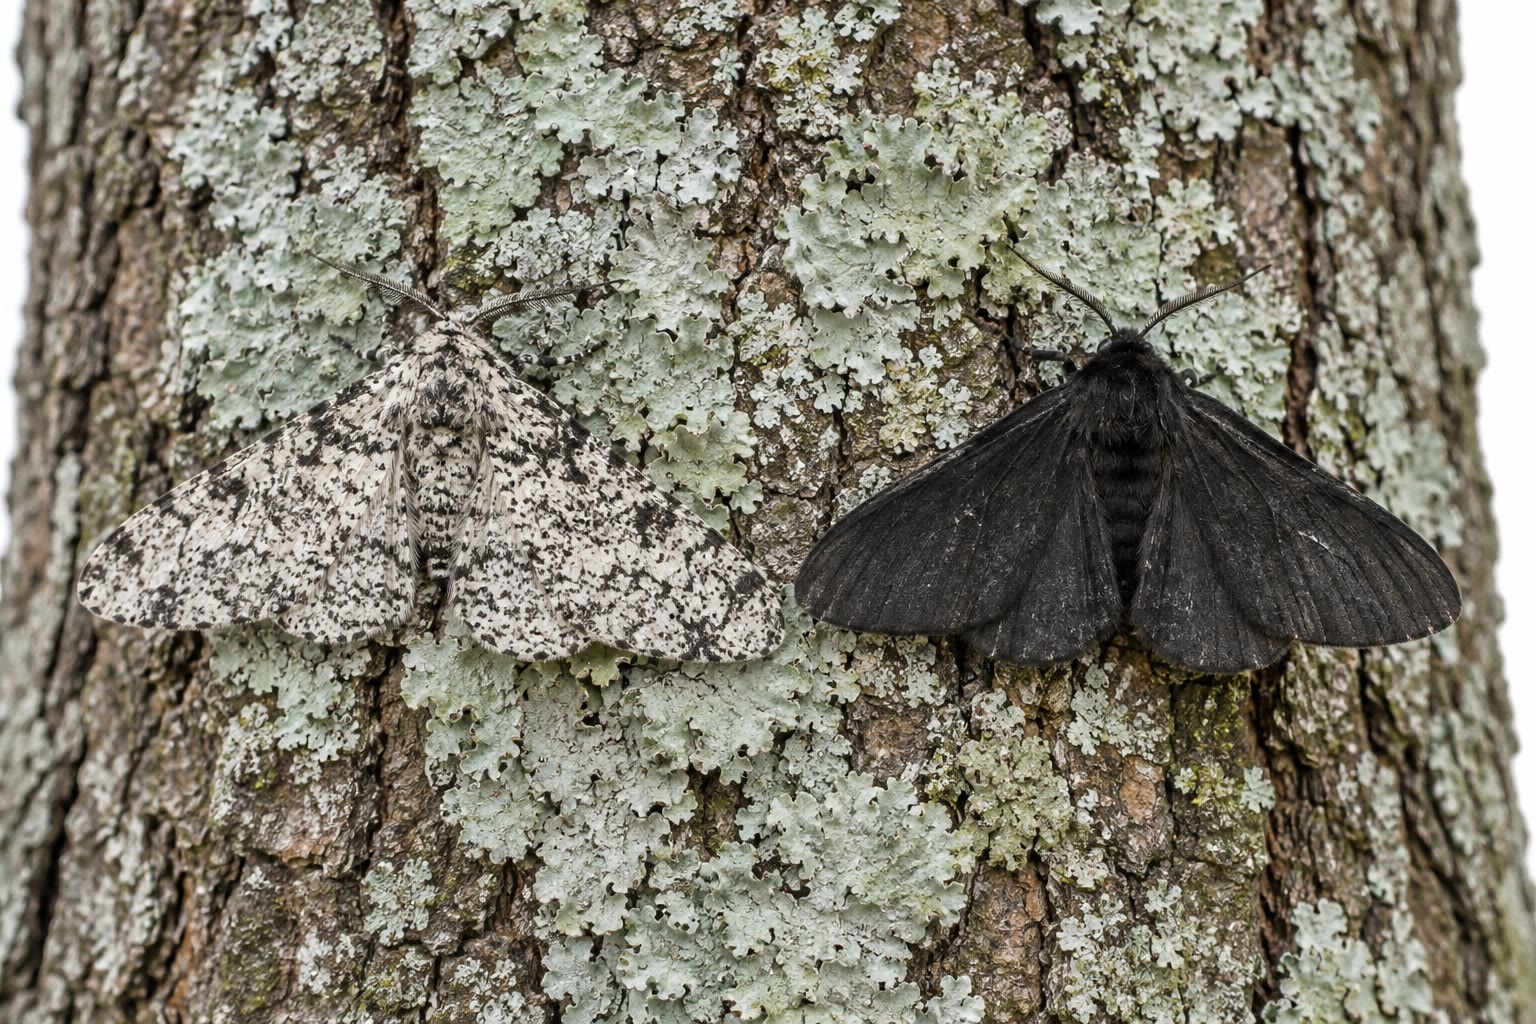
\includegraphics[width=0.46\linewidth]{images/book4/ai/b4-22-peppered-moths.jpg}\hspace{0.04\linewidth}
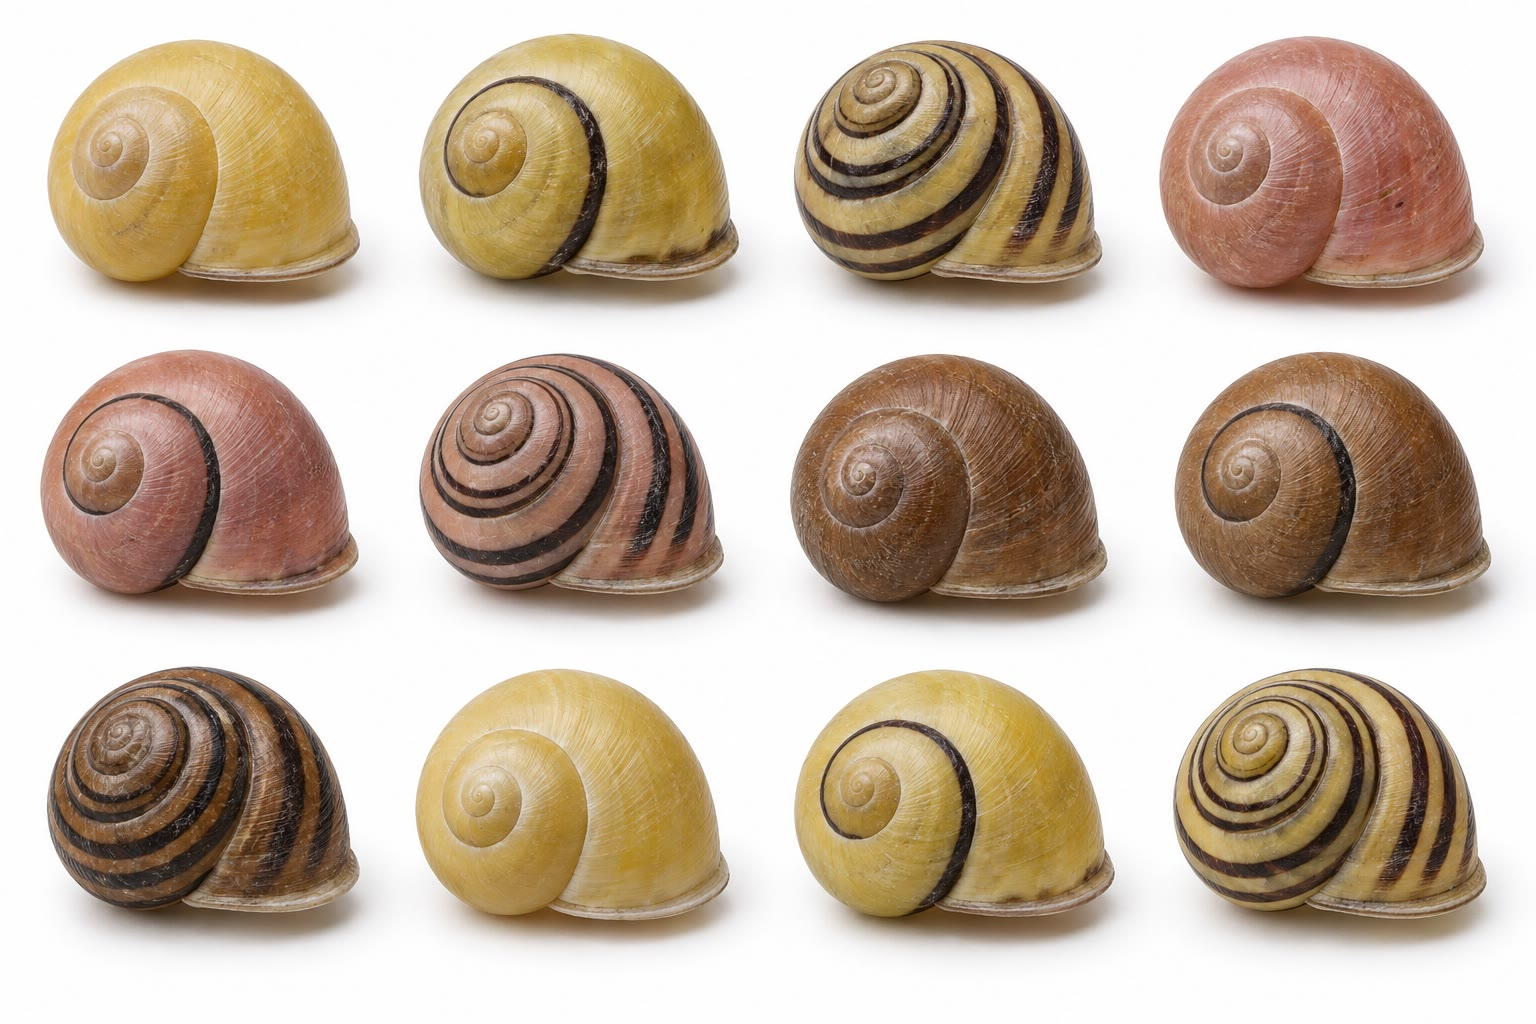
\includegraphics[width=0.46\linewidth]{images/book4/ai/b4-22-banded-snails.jpg}

{\small Links: de twee vormen van de berkenspanner op korstmos ---
welke een vogel vindt, hangt af van de schors. Rechts: het
schelppolymorfisme van de gewone tuinslak, met kleuren en banden die in elke
populatie in stand worden gehouden door roofdieren die de gewone vorm leren herkennen.}
\end{omfigure}

\section{Opgaven}

\begin{exercise}[$\star$]\label{exo:b2:population-genetics:1}
In een steekproef van 1000 mensen zijn er 640 $MM$, 320 $MN$ en 40 $NN$.
Bereken de \omterm{def:b2:population-genetics:frequencies}{allelfrequenties} en de verwachtingen volgens Hardy--Weinberg.
Is de populatie in evenwicht?
\end{exercise}

\begin{exercise}[$\star$]\label{exo:b2:population-genetics:2}
Albinisme is \omterm{def:b2:meiosis-heredity:vocabulary}{recessief} en treft één persoon op \num{20000}.
Bereken de \omterm{def:b2:population-genetics:frequencies}{allelfrequentie} en de dragersfrequentie.
\end{exercise}

\begin{exercise}[$\star$]\label{exo:b2:population-genetics:3}
Definieer \omterm{def:b2:population-genetics:fitness}{fitness}, \omterm{def:b2:population-genetics:fitness}{selectiecoëfficiënt} en \omterm{thm:b2:population-genetics:heritability}{erfelijkheidsgraad}, en noem de
vijf krachten die \omterm{def:b2:population-genetics:frequencies}{allelfrequenties} veranderen.
\end{exercise}

\begin{exercise}[$\star$]\label{exo:b2:population-genetics:4}
Geef van gerichte, stabiliserende en \omterm{prop:b2:population-genetics:kinds}{balancerende selectie} elk een voorbeeld,
met telkens de selecterende factor.
\end{exercise}

\begin{exercise}[$\star\star$]\label{exo:b2:population-genetics:5}
Een letaal \omterm{def:b2:meiosis-heredity:vocabulary}{recessief} \omterm{def:b2:meiosis-heredity:vocabulary}{allel} heeft frequentie $0.02$. Hoeveel
generaties duurt het om die te halveren? Om $0.001$ te bereiken? Wat zegt dit
over het effect van het verhinderen dat getroffenen zich voortplanten?
\end{exercise}

\begin{exercise}[$\star\star$]\label{exo:b2:population-genetics:6}
Bereken met $w_{AA} = 1$, $w_{Aa} = 1$, $w_{aa} = 0.8$ en $p = 0.3$
$\bar w$, $p'$ en $\Delta p$. Herhaal voor $p = 0.9$. Waarom is de
tweede verandering zoveel kleiner?
\end{exercise}

\begin{exercise}[$\star\star$]\label{exo:b2:population-genetics:7}
De sikkelcelhomozygoot heeft in een malariagebied $w = 0.2$ en de normale
\omterm{def:b2:meiosis-heredity:vocabulary}{homozygoot}
$w = 0.88$, de heterozygoten $w = 1$. Bereken de
evenwichtsfrequentie van het sikkelcelallel en de fractie van de kinderen die
in evenwicht met de ziekte wordt geboren.
\end{exercise}

\begin{exercise}[$\star\star$]\label{exo:b2:population-genetics:8}
Een \omterm{def:b2:meiosis-heredity:vocabulary}{recessief} \omterm{prop:b2:meiosis-heredity:extensions}{letaal allel} ontstaat door \omterm{def:b2:genome-diversification:mutation}{mutatie} met $\mu = \qty{2e-5}{}$ per
gameet. Bereken zijn evenwichtsfrequentie en de fractie getroffen geboorten.
Een \omterm{def:b2:meiosis-heredity:vocabulary}{dominant} \omterm{prop:b2:meiosis-heredity:extensions}{letaal allel} (vóór de voortplanting) met dezelfde snelheid:
welke fractie van de geboorten?
\end{exercise}

\begin{exercise}[$\star\star$]\label{exo:b2:population-genetics:9}
Een populatie van 50 zich voortplantende individuen begint met $H = 0.5$.
Bereken haar heterozygotie na 10, 50 en 200 generaties. Hoe
groot moet een populatie zijn om over 100 generaties \qty{90}{\%} van haar
heterozygotie te behouden?
\end{exercise}

\begin{exercise}[$\star\star\star$]\label{exo:b2:population-genetics:10}
Een eiland wordt gekoloniseerd door 10 vogels uit een populatie op het vasteland
waarin een \omterm{def:b2:meiosis-heredity:vocabulary}{allel} frequentie $0.1$ heeft. Bereken de kans dat
het \omterm{def:b2:meiosis-heredity:vocabulary}{allel} bij de stichters ontbreekt, en de kans dat het op het eiland
uiteindelijk gefixeerd raakt als het in één kopie aanwezig is.
Vergelijk met het vasteland.
\end{exercise}

\begin{exercise}[$\star\star\star$]\label{exo:b2:population-genetics:11}
De melkgift heeft $h^{2} = 0.3$ en een standaardafwijking van
\qty{1000}{L}. Een fokker houdt de beste \qty{20}{\%} van de koeien als
moeders (hun gemiddelde ligt $1.4$ standaardafwijkingen boven dat van de
kudde). Bereken de respons per generatie. Als stieren uit de
beste \qty{1}{\%} worden gekozen (gemiddelde $2.7$ standaardafwijkingen erboven), wat is dan de
respons? Waarom vertraagt de respons na veel generaties?
\end{exercise}

\begin{exercise}[$\star\star\star$]\label{exo:b2:population-genetics:12}
``Selectie is blind voor wat ze niet kan zien.'' Bespreek, met het
recessieve \omterm{def:b2:meiosis-heredity:vocabulary}{allel} in heterozygoten, de neutrale \omterm{def:b2:genome-diversification:mutation}{mutatie} en het
kenmerk met een \omterm{thm:b2:population-genetics:heritability}{erfelijkheidsgraad} nul, waarop selectie wel en niet kan
inwerken.
\end{exercise}

\section{Vraagstuk: de vlinder, het eiland en de kudde}

\begin{problem}[{Weekendvraagstuk --- de opkomst van de berkenspanner berekend
met de selectievergelijking, de drift en inteelt van een stichterspopulatie
gevolgd, een mutatie-selectie-evenwicht opgesteld, en een fokprogramma
voorspeld, met als besluit de selectiecoëfficiënt van de vlinder, de
heterozygotie van het eiland en de winst van de kudde}]
\label{pb:b2:population-genetics:1}
Berkenspanner: melanistisch \omterm{def:b2:meiosis-heredity:vocabulary}{allel} $M$ \omterm{def:b2:meiosis-heredity:vocabulary}{dominant}, frequentie $p_0 = 0.001$
in 1848; \qty{90}{\%} van de vlinders melanistisch 50 generaties later; neem aan
$w_{MM} = w_{Mm} = 1$ en $w_{mm} = 1 - s$. Eiland: gesticht door 12
vogels van een vasteland waar $H = 0.4$ en een \omterm{def:b2:meiosis-heredity:vocabulary}{recessief} schadelijk
\omterm{def:b2:meiosis-heredity:vocabulary}{allel} $q = 0.05$ heeft; het eiland herbergt daarna 40 zich voortplantende
vogels. \omterm{def:b2:genome-diversification:mutation}{Mutatie}: $\mu = \qty{1e-5}{}$. Kudde: $h^{2} = 0.4$,
standaardafwijking \qty{800}{L}.

\medskip
\noindent\textbf{Deel I --- De vlinder.}
\begin{enumerate}
  \item Welke fractie van de vlinders was in 1848 melanistisch, en welke
        fractie van de $M$-allelen zat in heterozygoten?
  \item Toon aan dat, met $M$ \omterm{def:b2:meiosis-heredity:vocabulary}{dominant}, de frequentie van het lichte
        \omterm{def:b2:meiosis-heredity:vocabulary}{allel} voldoet aan $q' = q(1 - sq)/(1 - sq^{2})$.
  \item Bereken, uitgaande van $q_0 = 0.999$, $q$ na één generatie
        voor $s = 0.3$.
  \item \qty{90}{\%} melanistisch betekent $q^{2} = 0.1$. Wat is $q$ dan?
  \item Schat door proberen met de recursie (of de benadering
        $\Delta q \approx -sq^{2}p$ zolang $q$ dicht bij 1 ligt) het
        aantal generaties dat $s = 0.3$ nodig heeft om $q$ van $0.999$
        tot $0.32$ te brengen, en vergelijk met de waargenomen 50.
  \item Na de wetten voor schone lucht heeft de lichte vorm het voordeel: $s
        = 0.3$ tegen $mm$ wordt $s = 0.3$ tegen $M\_$. Toon aan
        dat $\Delta p = -spq^{2}/\bar w$, en leg uit waarom de terugkeer
        van de lichte vorm eerst traag is en eindigt in een exponentiële
        afname van $M$, terwijl de opkomst exponentieel begon en
        in een slakkengang eindigde.
\end{enumerate}

\medskip
\noindent\textbf{Deel II --- Het eiland.}
\begin{enumerate}[resume]
  \item Bereken de kans dat geen van de 12 stichters het schadelijke \omterm{def:b2:meiosis-heredity:vocabulary}{allel}
        draagt.
  \item Bereken de verwachte heterozygotie na de stichtersgeneratie
        (getrokken uit $H = 0.4$ door 12 individuen, d.w.z.\ 24
        genkopieën).
  \item Bereken de heterozygotie na 100 generaties bij $N =
        40$, als fractie van die van het vasteland.
  \item Een neutrale \omterm{def:b2:genome-diversification:mutation}{mutatie} verschijnt in één vogel. Bereken haar
        fixatiekans en de verwachte tijd tot fixatie als ze
        gefixeerd raakt.
  \item De eilandvogels paren willekeurig maar zijn allemaal verwant. Met
        $F = 1/(2N)$ die zich per generatie opstapelt tot ongeveer $0.3$ na
        30 generaties, bereken de frequentie van getroffen homozygoten
        voor het \omterm{def:b2:meiosis-heredity:vocabulary}{allel} met $q = 0.05$, met en zonder inteelt.
  \item Elke generatie komt er één vogel van het vasteland aan. Leg uit wat
        dit doet met de divergentie van het eiland en met zijn last.
\end{enumerate}

\medskip
\noindent\textbf{Deel III --- Het evenwicht.}
\begin{enumerate}[resume]
  \item Bereken de evenwichtsfrequentie van een \omterm{def:b2:meiosis-heredity:vocabulary}{recessief} \omterm{prop:b2:meiosis-heredity:extensions}{letaal allel} dat
        wordt aangevuld met $\mu = 10^{-5}$, en de fractie getroffen geboorten.
  \item Bereken hetzelfde voor $s = 0.1$ (een licht schadelijk
        \omterm{def:b2:meiosis-heredity:vocabulary}{recessief} \omterm{def:b2:meiosis-heredity:vocabulary}{allel}).
  \item Bereken het evenwicht voor een \omterm{def:b2:meiosis-heredity:vocabulary}{dominant} \omterm{def:b2:meiosis-heredity:vocabulary}{allel} met
        \omterm{def:b2:meiosis-heredity:vocabulary}{heterozygoot} nadeel $hs = 0.05$.
  \item De geneeskunde geneest de letale aandoening, zodat $s$ daalt tot $0.1$. Hoe
        verandert het evenwicht, en hoelang (in orde van grootte) doet de
        populatie erover om daar te komen?
  \item Het genoom heeft \num{20000} genen die elk met $10^{-5}$ muteren tot
        een \omterm{def:b2:meiosis-heredity:vocabulary}{recessief} \omterm{prop:b2:meiosis-heredity:extensions}{letaal allel}. Hoeveel letale \omterm{def:b2:meiosis-heredity:vocabulary}{allelen} draagt een
        gemiddelde persoon in heterozygote toestand? (In
        evenwicht heeft elk locus $2\hat q$ kopieën per persoon.)
  \item Leg uit waarom dat aantal verenigbaar is met een gezonde
        populatie en waarom het een huwelijk tussen neef en nicht kostbaar maakt.
\end{enumerate}

\medskip
\noindent\textbf{Deel IV --- De kudde.}
\begin{enumerate}[resume]
  \item De fokker houdt de beste \qty{30}{\%} van de koeien (gemiddelde $1.16$
        standaardafwijkingen boven de kudde). Bereken het
        selectiedifferentieel in liters en de respons.
  \item Wat is na vijf generaties van dezelfde selectie de verwachte winst,
        en waarom zou de werkelijke winst kleiner kunnen zijn?
  \item Stieren leveren de helft van de genen en worden uit de beste
        \qty{2}{\%} gekozen ($2.4$ standaardafwijkingen). Bereken de respons
        wanneer koeien en stieren zoals hierboven worden geselecteerd (neem het
        gemiddelde van de twee differentiëlen).
  \item Een kudde waarin alle koeien klonen van één dier zijn: wat zijn
        $h^{2}$ en de respons? Wat zegt dat over de
        \omterm{thm:b2:population-genetics:heritability}{erfelijkheidsgraad}?
  \item Een vinkenpopulatie heeft $h^{2} = 0.7$ voor snaveldiepte en de
        droogte laat overlevenden achter met snavels die \qty{0.6}{mm} dieper
        zijn. Voorspel de volgende generatie.
  \item De fokker richt zich op een eigenschap met $h^{2} = 0.1$. Welk
        selectiedifferentieel, in standaardafwijkingen, geeft dezelfde
        respons als in vraag 19?
  \item Formuleer het resultaat: de $s$ van de vlinder en de tijd tot \qty{90}{\%}
        melanistisch, de heterozygotie van het eiland na 100 generaties,
        en de respons van de kudde per generatie.
\end{enumerate}
\end{problem}
